\begin{frame}{\glqq Entdeckung\grqq\ Dunkler Materie}
	\begin{itemize}
		\item Menschen schauen schon immer in den Himmel.
		\item Großteil dessen was das Universums ausmacht ist unbekannt. (Daten ESA, Planck Colaboration)
		\item Dunkle Materie als Lösung für zu schnelle Galaxien.
	\end{itemize}
%\begin{minipage}{.45\textwidth}
%	\begin{figure}
%		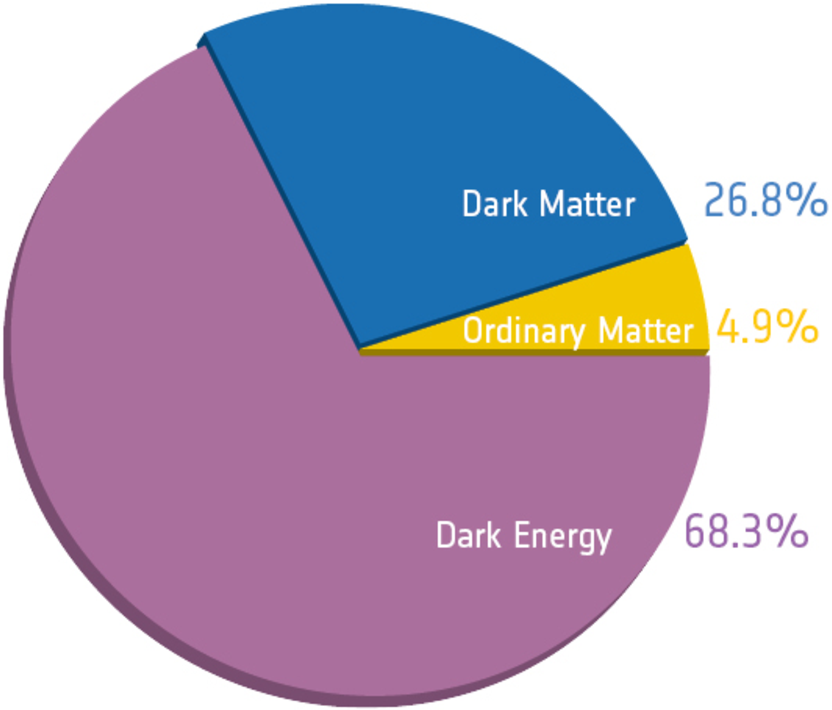
\includegraphics[width=\textwidth]{Bilder/EnergyUniverse.pdf}
%		\caption{Energieverteilung im Universum (ESA, Planck Colaboration)}
%	\end{figure}
%\end{minipage}
%\hfill
%\begin{minipage}{.45\textwidth}
	\begin{figure}[H]
		\resizebox{.5\textwidth}{!}{
			\begin{tikzpicture}
\tikzstyle{centerArrow}=[decoration={
    markings,
    mark=at position 0.5 with {\fill (2pt,0)--(-2pt,2.31pt)--(-2pt,-2.31pt)--cycle;}}]
\begin{scope}
\def\xmove{2.5}
\def\ymove{1.25}
\def\centerSize{0.15}
\node [fill, circle,inner sep=\centerSize cm] (tCenter)  {};
\node (upperLeft) at (-\xmove,\ymove) {$\chi$};
\node (upperRight) at (\xmove,\ymove) {$\chi$};
\node (lowerLeft) at (-\xmove,-\ymove) {$N$};
\node (lowerRight) at (\xmove,-\ymove) {$N$};
\draw [centerArrow,postaction={decorate}]  (upperLeft) -- (tCenter) ;
\draw [centerArrow,postaction={decorate}]  (lowerLeft) -- (tCenter) ;
\draw [centerArrow,postaction={decorate}]  (tCenter) -- (upperRight) ;
\draw [centerArrow,postaction={decorate}]  (tCenter) -- (lowerRight) ;
\end{scope}
\end{tikzpicture}
		}
%		\captionsetup{width=\textwidth}
		\caption{Direct Detection: Streuung eines DM-Teilchens am Atomkern.}
	\end{figure}
%\end{minipage}
\end{frame}
\begin{frame}
	\begin{figure}
		\centering
		\begin{tikzpicture}
			\pie[
				color={yellow, green, blue!60},
				radius=2,
				text=legend,
				explode={0,0,0.3}
				]{4.9/Gewöhnliche Materie, 26.8/ Dunkle Materie, 68.3/ Dunkle Energie}
		\end{tikzpicture}
		\caption{Energieverteilung im Universum (ESA, Planck Colaboration 2013)}
	\end{figure}
\end{frame}